\documentclass[../master/master.tex]{subfiles}
\begin{document}
Once the algorithms had been implemented, we needed to find some inputs to conduscct our experiments. We found large datasets

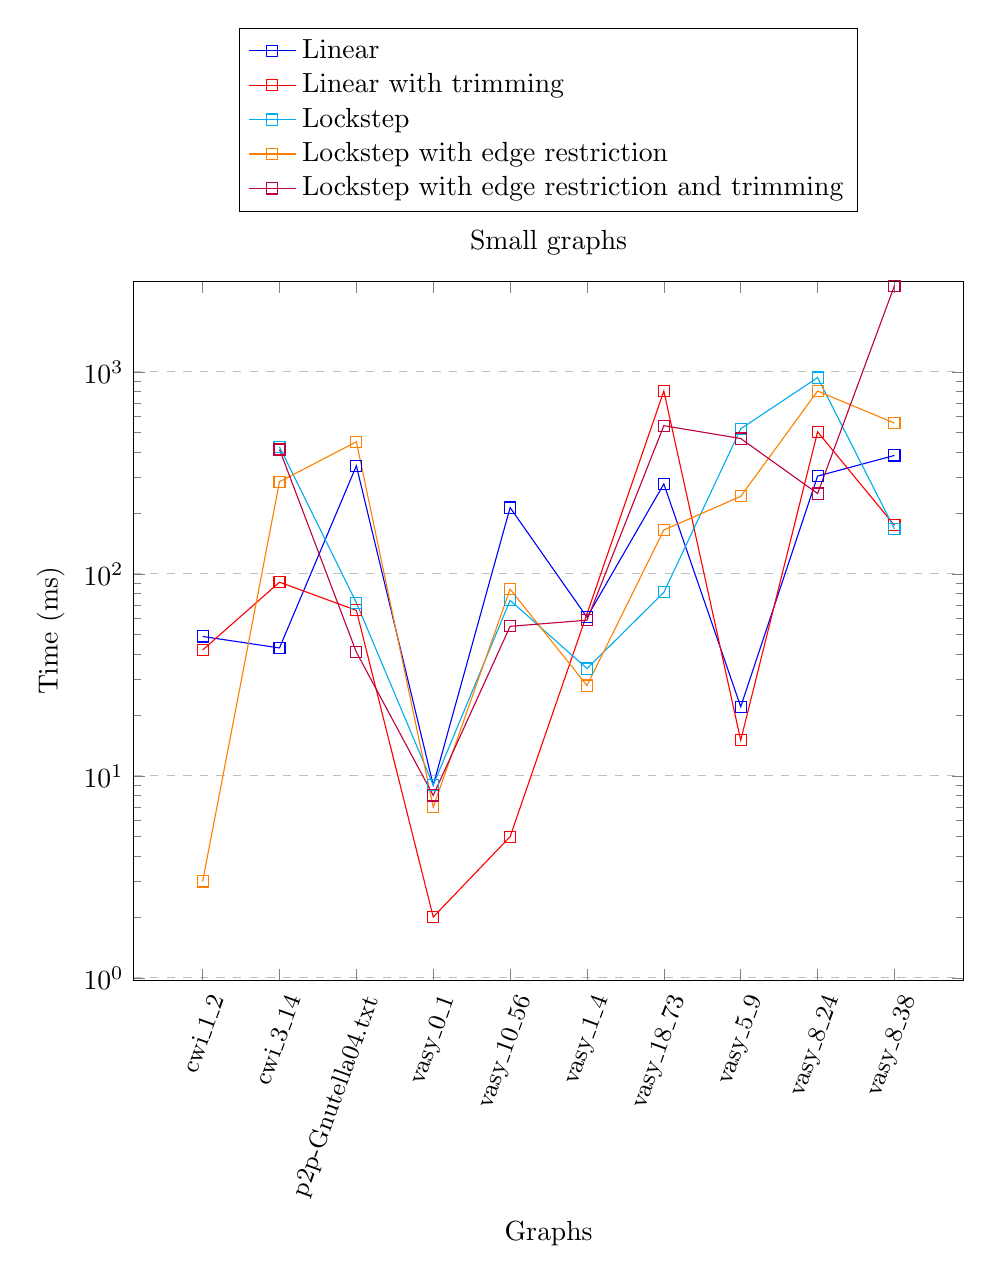
\begin{tikzpicture}
  \begin{axis}[
    width=\textwidth,
    symbolic x coords={cwi\_1\_2, cwi\_3\_14, p2p-Gnutella04.txt, vasy\_0\_1, vasy\_10\_56, vasy\_1\_4, vasy\_18\_73, vasy\_5\_9, vasy\_8\_24, vasy\_8\_38},
    x tick label style = {font = \small, align = center, rotate = 70, anchor = north east},
    title={Small graphs},
    xlabel={Graphs},
    ylabel={Time (ms)},
    ymin=0, ymax=2800,
    legend style={at={(0.5,1.1)},anchor=south,legend cell align=left},
    ymajorgrids=true,
    grid style=dashed,
    ymode=log,
    log basis y={10}
]

\addplot[color=blue,mark=square,]coordinates {(cwi\_1\_2, 49)(cwi\_3\_14, 43)(p2p-Gnutella04.txt, 343)(vasy\_0\_1, 9)(vasy\_10\_56, 213)(vasy\_1\_4, 61)(vasy\_18\_73, 279)(vasy\_5\_9, 22)(vasy\_8\_24, 305)(vasy\_8\_38, 386)};
\addplot[color=red,mark=square,]coordinates {(cwi\_1\_2, 42)(cwi\_3\_14, 91)(p2p-Gnutella04.txt, 066)(vasy\_0\_1, 2)(vasy\_10\_56, 005)(vasy\_1\_4, 00)(vasy\_18\_73, 804)(vasy\_5\_9, 15)(vasy\_8\_24, 505)(vasy\_8\_38, 174)}; 
\addplot[color=cyan,mark=square,]coordinates {(cwi\_1\_2, 0)(cwi\_3\_14, 426)(p2p-Gnutella04.txt, 072)(vasy\_0\_1, 9)(vasy\_10\_56, 74)(vasy\_1\_4, 34)(vasy\_18\_73, 081)(vasy\_5\_9, 523)(vasy\_8\_24, 938)(vasy\_8\_38, 167)};
\addplot[color=orange,mark=square,]coordinates {(cwi\_1\_2, 3)(cwi\_3\_14, 286)(p2p-Gnutella04.txt, 451)(vasy\_0\_1, 7)(vasy\_10\_56, 84)(vasy\_1\_4, 28)(vasy\_18\_73, 165)(vasy\_5\_9, 242)(vasy\_8\_24, 804)(vasy\_8\_38, 558)};
\addplot[color=purple,mark=square,]coordinates {(cwi\_1\_2, 0)(cwi\_3\_14, 413)(p2p-Gnutella04.txt, 41)(vasy\_0\_1, 8)(vasy\_10\_56, 55)(vasy\_1\_4, 59)(vasy\_18\_73, 542)(vasy\_5\_9, 468)(vasy\_8\_24, 250)(vasy\_8\_38, 2674)}; \legend{Linear, Linear with trimming, Lockstep, Lockstep with edge restriction, Lockstep with edge restriction and trimming}
\end{axis}
\end{tikzpicture}

\begin{tikzpicture}
  \begin{axis}[
    width=\textwidth,
    height = \textheight,
    symbolic x coords={vasy\_116\_368, vasy\_157\_297, vasy\_52\_318, vasy\_720\_390, vasy\_83\_325, web-Stanford.txt},
    x tick label style = {font = \small, align = center, rotate = 70, anchor = north east},
    xtick=data,
    title={Large graphs},
    xlabel={Graphs},
    ylabel={Time (ms)},
    ymin=0, ymax=1000000,
    legend pos = north east,
    %legend style={at={(0.5,1.02)},anchor=south,legend cell align=left},
    ymajorgrids=true,
    grid style=dashed,
    ymode=log,
    log basis y={100}
    ]
\addplot[color=blue,mark=square,]coordinates {(vasy\_116\_368, 46786)(vasy\_157\_297, 53563)(vasy\_52\_318, 5608)(vasy\_720\_390, 7531)(vasy\_83\_325, 3562)(web-Stanford.txt, 0)}; 
\addplot[color=red,mark=square,]coordinates {(vasy\_116\_368, 49855)(vasy\_157\_297, 91313)(vasy\_52\_318, 7534)(vasy\_720\_390, 3638)(vasy\_83\_325, 5691)(web-Stanford.txt, 0)}; 
\addplot[color=cyan,mark=square,]coordinates {(vasy\_116\_368, 0)(vasy\_157\_297, 542037)(vasy\_52\_318, 17469)(vasy\_720\_390, 32579)(vasy\_83\_325, 936)(web-Stanford.txt, 0)}; 
\addplot[color=orange,mark=square,]coordinates {(vasy\_116\_368, 0)(vasy\_157\_297, 137648)(vasy\_52\_318, 3209)(vasy\_720\_390, 59329)(vasy\_83\_325, 034)(web-Stanford.txt, 216873)};
\addplot[color=purple,mark=square,]coordinates {(vasy\_116\_368, 0)(vasy\_157\_297, 0)(vasy\_52\_318, 5463)(vasy\_720\_390, 7275)(vasy\_83\_325, 205)(web-Stanford.txt, 34071)};
\legend{Linear, Linear with trimming, Lockstep, Lockstep with edge restriction, Lockstep with edge restriction and trimming}
\end{axis}
\end{tikzpicture}

\end{document}
%%% Local Variables:
%%% mode: latex
%%% TeX-master: "../master/master"
%%% End:
